\documentclass[article,12pt,a4paper,oneside,brazil]{abntex2}
\usepackage[utf8]{inputenc}
\usepackage{pacotes}
\usepackage{booktabs}
\geometry{left=3cm,right=2cm,top=2.5cm,bottom=2.5cm}
\hypersetup{pdftitle={Estimativa exploratória de permanência em assentos de um restaurante universitário},pdfauthor={Bruno Sime Ferreira Nunes},colorlinks=true,linkcolor=black,citecolor=black,urlcolor=blue}
\setlength{\parindent}{1.2em}
\setlength{\parskip}{2pt}
\setlength{\abovecaptionskip}{5pt}
\setlength{\belowcaptionskip}{3pt}
\captionsetup{font=small}
\pagestyle{plain}
\newcommand{\fontedados}[1]{\par\vspace{3pt}{\footnotesize Fonte: #1.}\par}
\makepagestyle{artigoUFPR}
\makeoddfoot{artigoUFPR}{}{\small\thepage}{}
\makeevenfoot{artigoUFPR}{}{\small\thepage}{}
\begin{document}
\pagestyle{artigoUFPR}
\SingleSpacing
\begin{center}
{\small UNIVERSIDADE FEDERAL DO PARANÁ\\Visão Computacional e Percepção --- Prof. Eduardo Todt}\par
\vspace{0.35cm}
{\Large\bfseries Estimativa exploratória de permanência em assentos de um restaurante universitário}\par
\vspace{0.2cm}
{\normalsize Bruno Sime Ferreira Nunes}\par
{\small Curitiba, 2026}
\end{center}
\noindent\textbf{Resumo.} Este trabalho estima a permanência sentada em uma amostra de assento de restaurante universitário e avalia quatro configurações de visão computacional. Uma gravação de aproximadamente três horas, no período informado das 11h às 14h, foi processada com YOLO11-Pose e BoT-SORT. Todas as configurações percorreram os 107.981 quadros do arquivo. A associação geométrica contempla quatro regiões de assento; a conferência temporal aprofundada concentra-se em uma delas, S2, escolhida por visibilidade. Uma revisão visual por IA identificou cinco sessões completas e uma censurada ao final. Usando pontos médios dos intervalos de sentar e levantar, obteve-se média nominal de \textbf{16 min 16 s}, mediana de 14 min 10 s e durações de 5 min 44 s a 25 min 02 s. A triagem utiliza quadros de um minuto, a conferência interna dez segundos e o refinamento de eventos dois segundos. O resultado descreve apenas as sessões completas observáveis desse assento. A amostra pequena, as pausas potencialmente não observadas e a ausência de validação humana independente impedem generalizar a média ao RU inteiro ou declarar precisão operacional do método automático.

\noindent\textbf{Palavras-chave:} visão computacional; rastreamento; estimação de pose; ocupação de assentos; análise de vídeo.

\section{Introdução}
Estimar a permanência à mesa pode apoiar estudos de utilização de um restaurante universitário. A câmera fixa permite acompanhar a mesma região durante o almoço, mas a cena contém pessoas em circulação, oclusões pelas mesas e substituição de ocupantes. Assim, acompanhar uma caixa ao longo do vídeo não demonstra que a pessoa permaneceu sentada durante todo esse intervalo.

O rastreamento de múltiplos objetos associa detecções entre quadros. O BoT-SORT combina componentes de movimento e, opcionalmente, aparência e compensação de câmera \cite{aharon2022}. Entretanto, bons resultados em conjuntos de pedestres não garantem continuidade em pessoas sentadas parcialmente encobertas. A própria associação de detecções de baixa confiança busca reduzir perdas e trajetórias fragmentadas \cite{zhang2022}.

O objetivo é obter uma média descritiva de sessões completas por revisão visual, comparar quatro configurações automáticas e distinguir identificadores de permanências reais. A contribuição combina execução reproduzível e uma tabela temporal auditável. O estudo é de caso: a conferência foi realizada por IA, sem validação humana independente ou teste separado.

\noindent\textbf{Código e materiais:} \url{https://github.com/bruno-sime/computerVision}. Os arquivos desta entrega estão organizados para publicação nesse repositório.

\clearpage
\section{Materiais e desenho experimental}
\subsection{Gravação e integridade}
Utilizou-se um MP4/H.264 de uma sexta-feira, com 1.562.926.905 bytes, resolução de $1280\times720$ pixels, taxa próxima de 10 quadros/s e duração de 10.798,357 s. O início às 11h foi informado pelo responsável pelo arquivo; o término corresponde aproximadamente a 13h59min58s. O campo visível da câmera não cobre necessariamente todos os assentos do estabelecimento.

A contagem de 107.981 quadros lidos coincidiu com a esperada em todas as execuções. A maior separação entre timestamps de pacotes do arquivo foi 0,140 s. O hash SHA-256 calculado localmente coincidiu com o registrado no servidor; o valor completo consta do manifesto. Essas verificações comprovam integridade entre as cópias e cobertura do arquivo, sem demonstrar ausência de edição anterior à exportação.

\subsection{Modelos e parâmetros}
Foram usados pesos pré-treinados de YOLO11m-pose e YOLO11x-pose, sem treinamento ou ajuste fino no vídeo. A família oferece detecção de pontos corporais \cite{ultralytics11}. As inferências utilizaram entrada 1280, confiança mínima 0,15, IoU 0,60 e precisão FP16. O BoT-SORT operou sem ReID e sem compensação global de movimento, pois a câmera é fixa. Não houve reconhecimento facial.

\begin{table}[H]
\centering
\caption{Condições experimentais; alteração de uma variável em relação a A.}
\label{tab:configs}
\begin{tabular}{clccp{4.8cm}}
\toprule
Condição & Modelo & Obs./s & Buffer & Comparação com A\\
\midrule
A & YOLO11x-pose & 2 & 15 s & Referência\\
B & YOLO11m-pose & 2 & 15 s & Tamanho do modelo\\
C & YOLO11x-pose & 5 & 15 s & Frequência de observação\\
D & YOLO11x-pose & 2 & 5 s & Tolerância a perdas\\
\bottomrule
\end{tabular}
\fontedados{configurações efetivamente executadas}
\end{table}
O buffer foi convertido para número de observações, preservando a duração nominal ao mudar a frequência. Ele mantém trajetórias perdidas disponíveis para associação; não autoriza contabilizar o intervalo como tempo sentado. O estudo não é um experimento fatorial completo.

O servidor Ubuntu possuía NVIDIA RTX 6000 Ada de 48 GB, PyTorch 2.15.0 e Ultralytics 8.4.214. B e C foram executados simultaneamente, enquanto A e D tiveram execuções separadas. Por isso, os tempos registrados são operacionais, e não uma comparação controlada de eficiência entre modelos.

\clearpage
\section*{Exemplos visuais da gravação}
As imagens apresentam o enquadramento real e duas posturas no assento S2. Máscaras e pixelização ocultam detalhes faciais, sem alteração da postura corporal visível. Os instantes ilustrativos não substituem as janelas de marcação dos eventos usadas no cálculo da média.
\begin{figure}[H]\centering
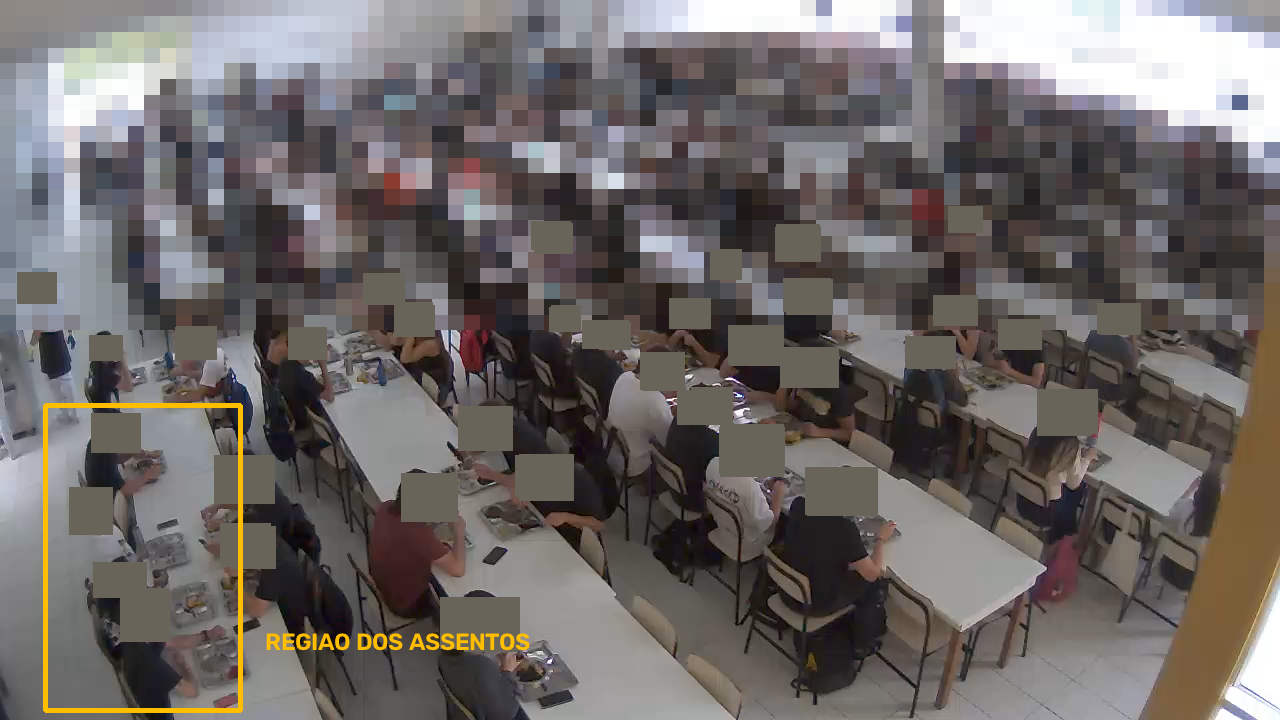
\includegraphics[width=0.95\textwidth]{figuras/exemplos/enquadramento.png}
\caption{Enquadramento em 3.600,086 s, aproximadamente às 12h, com a região dos assentos demarcada. A região distante foi pixelizada e detalhes faciais foram ocultados.}
\fontedados{quadro real extraído da gravação e editado apenas para ocultação e demarcação}
\end{figure}
\begin{figure}[H]\centering
\begin{minipage}{0.44\textwidth}\centering
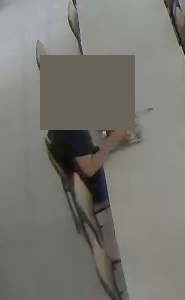
\includegraphics[height=6cm]{figuras/exemplos/sentado.png}\\
\small (a) Sentado: 11h35min20s.
\end{minipage}\hfill
\begin{minipage}{0.44\textwidth}\centering
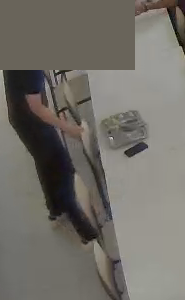
\includegraphics[height=6cm]{figuras/exemplos/em_pe.png}\\
\small (b) Em pé: 11h41min02s.
\end{minipage}
\caption{Exemplos da sessão E2 no assento S2. Os recortes preservam a cadeira e a postura, com a região da cabeça ocultada. A marcação temporal considera as janelas dos eventos e não apenas estes quadros.}
\fontedados{recortes reais dos instantes 2.120 e 2.462 s da gravação}
\end{figure}

\clearpage
\section{Associação aos assentos e conferência visual}
\subsection{Hipótese geométrica de ocupação}
A etapa automática contempla quatro regiões próximas à câmera, na lateral esquerda da mesa em primeiro plano. A seleção prioriza visibilidade e mantém as regiões fixas durante as três horas, sem amostragem aleatória de usuários. As posições e os parâmetros estão em \texttt{dataset/assentos.json}.

Calcula-se o centro ponderado dos quadris, exigindo confiança mínima 0,40 em ao menos um quadril e um ombro. Os ombros devem estar 25 pixels acima do quadril. A distância ao centro da região $j$ é
\begin{equation}
d_j=\left(\frac{x-x_j}{27}\right)^2+\left(\frac{y-y_j}{20}\right)^2.
\end{equation}
Aceitam-se candidatos com $d_j\leq1$. A associação gulosa prioriza menor distância, sem reutilizar ID ou assento na observação. Essa geometria é uma hipótese de ocupação, não prova de contato com a cadeira. O assento S2 usa centro aproximado $(118,595)$ pixels para o quadril.

\subsection{Pós-processamento automático}
Uma grade comum de 5 s reduz a resolução temporal das quatro condições nesta etapa. Extrai-se a mediana CIELAB do torso entre ombros e quadris. Distância de cor superior a 35 por três observações sinaliza possível troca de ocupante frente à mediana das seis últimas cores aceitas. A aparência é da roupa, sem reconhecimento facial.

A heurística tolera duas posições sem detecção, encerra na terceira ausência e mantém intervalos de pelo menos 60 s. Seu fim corresponde à última observação aceita mais 5 s. Esses candidatos incluem lacunas toleradas e não são utilizados diretamente para calcular a média principal. Roupas parecidas, postura e pontos corporais incorretos podem unir ou dividir episódios.

\subsection{Referência temporal e cálculo da média}
A revisão aprofundada acompanha o assento S2 em todo o arquivo. A triagem visual em quadros separados por 60 s localiza sessões com pelo menos um minuto. Os episódios identificados são conferidos internamente em quadros a cada 10 s, usando o contexto da cadeira e a continuidade visual do ocupante. Não se detectaram pausas em pé nos instantes internos aceitos; pausas breves entre amostras podem passar despercebidas.

O início é a transição para sentar e o fim é levantar. Janelas com quadros separados por 2 s delimitam cada evento entre o último estado anterior e o primeiro posterior observável. Quando a postura ou uma oclusão tornam o instante ambíguo, conserva-se um intervalo maior, de até 10 s. Usa-se seu ponto médio para a duração nominal. Cinco sessões têm ambas as bordas observáveis. A sexta começa no vídeo, mas permanece em andamento ao final e é excluída da média de completas.

A revisão foi executada pelo assistente de IA. Ela constitui uma referência visual assistida e auditável, sem atribuição de conferência humana ao autor. Os intervalos, critérios e proveniência constam do CSV e do script de cálculo. A média descreve permanência sentada observável na resolução adotada, sem alegação de verificação contínua quadro a quadro ou validação independente.

\clearpage
\section{Resultados das quatro configurações}
A Tabela~\ref{tab:resultados} resume as observações rastreadas. Cada ID é um identificador do algoritmo, não uma pessoa distinta. O intervalo de um ID é a diferença entre sua última e primeira observação e pode incluir oclusões, deslocamento ou associação incorreta.

\begin{table}[H]
\centering
\caption{Resultados descritivos do rastreamento no arquivo completo.}
\label{tab:resultados}
\small
\begin{tabular}{crrrrr}
\toprule
Cond. & Imagens & IDs & IDs $<30$ s & IDs $\geq10$ min & Det./imagem\\
\midrule
A & 21.597 & 4.280 & 70,89\% & 161 & 26,667\\
B & 21.597 & 4.883 & 69,96\% & 138 & 26,166\\
C & 53.992 & 7.203 & 76,83\% & 122 & 27,326\\
D & 21.597 & 5.677 & 78,33\% & 141 & 26,365\\
\bottomrule
\end{tabular}
\fontedados{auditoria integral dos registros JSONL}
\end{table}
B emitiu 14,1\% mais IDs que A; C, 68,3\%; e D, 32,6\%. A maior frequência não levou a menos IDs, e a menor tolerância aumentou sua proporção de intervalos breves. Essas diferenças são compatíveis com mudanças na observação de pessoas transitórias e na fragmentação, mas não permitem separar as causas sem referência de identidade. Menos IDs tampouco prova melhor rastreamento, pois associações incorretas podem unir pessoas diferentes.

\begin{figure}[H]
\centering
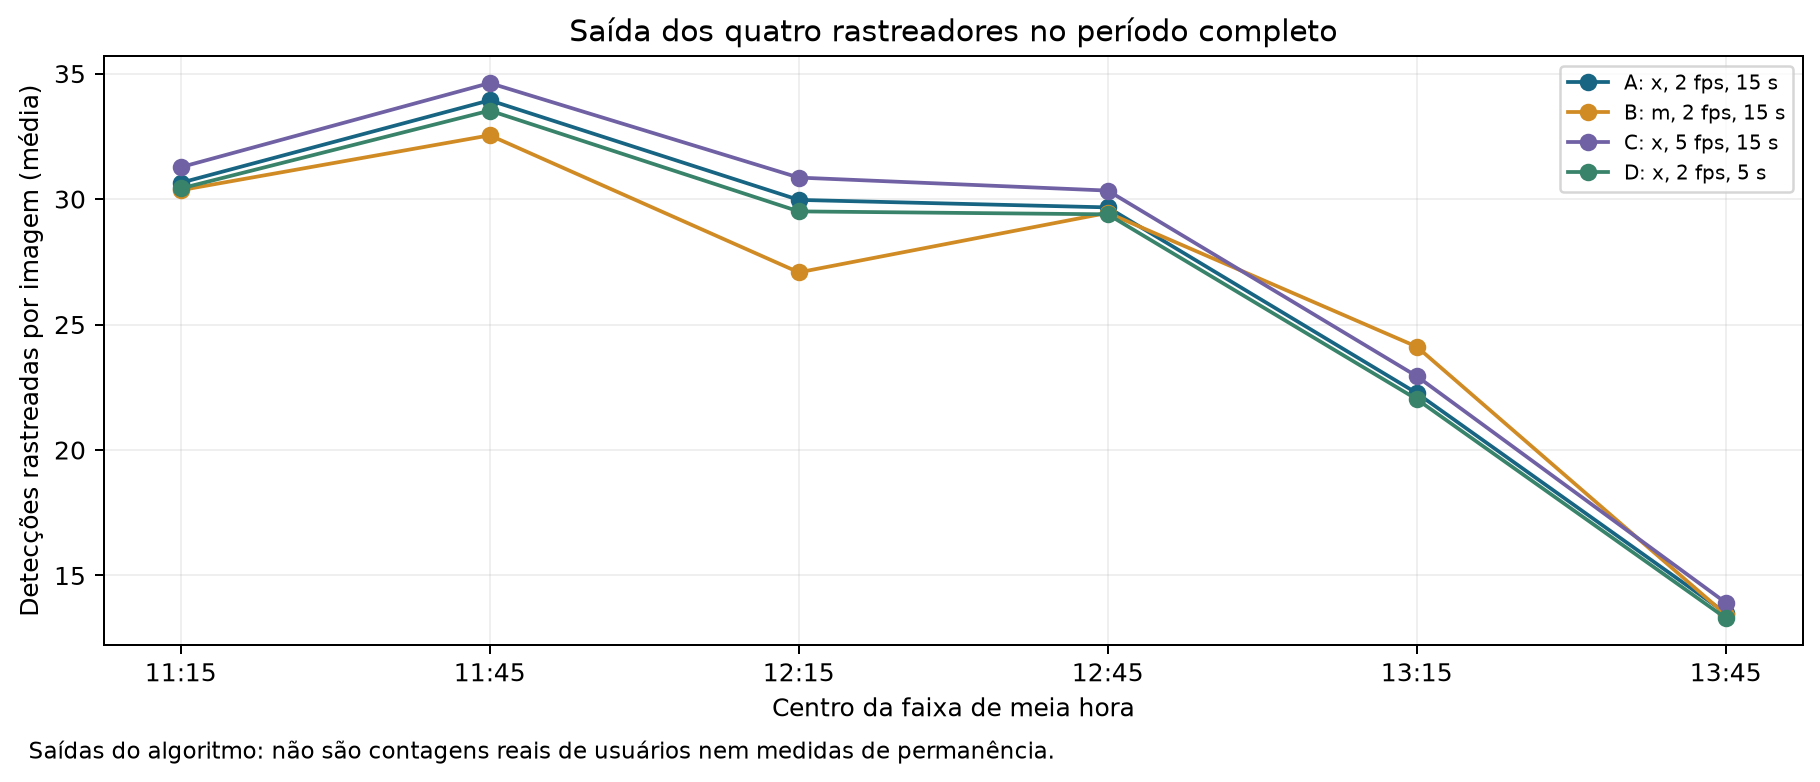
\includegraphics[width=\textwidth]{figuras/deteccoes_por_faixa.png}
\caption{Média das detecções rastreadas em faixas de 30 minutos. A tendência temporal não corresponde à ocupação real do restaurante.}
\label{fig:faixas}
\fontedados{registros das quatro execuções}
\end{figure}
A queda no fim do período é coerente com as amostras visuais de esvaziamento. Entretanto, as imagens mostram perdas no fundo e oclusões no primeiro plano. Não foram calculados precisão, recall, IDF1, MOTA ou HOTA, pois não há anotações independentes adequadas para essas métricas.

Os tempos observados foram 364,6 s (A), 387,3 s (B), 912,9 s (C) e 357,1 s (D). A concorrência de B e C e o maior número de observações em C impedem interpretar esses valores como velocidade isolada das arquiteturas. Todos os registros e tabelas de IDs foram conferidos entre si.

\clearpage
\section{Média das sessões visualmente revisadas}
A Tabela~\ref{tab:media} apresenta todas as cinco sessões completas identificadas na revisão temporal do assento S2. Os horários são relativos ao início informado às 11h e representam pontos médios dos intervalos dos eventos. Cada linha corresponde a uma permanência do mesmo ocupante observável, sem usar a duração de um ID como referência.

\begin{table}[H]
\centering
\caption{Sessões completas revisadas por IA no assento S2.}
\label{tab:media}
\begin{tabular}{cllr}
\toprule
Sessão & Início nominal & Fim nominal & Duração nominal\\
\midrule
% BEGIN SESSOES REVISADAS
E1 & 11:13:42 & 11:27:52 & 14 min 10 s \\
E2 & 11:35:14 & 11:40:58 & 5 min 44 s \\
E3 & 11:41:54 & 12:06:56 & 25 min 02 s \\
E4 & 12:08:54 & 12:31:48 & 22 min 54 s \\
E5 & 12:33:57 & 12:47:27 & 13 min 30 s \\
% END SESSOES REVISADAS
\bottomrule
\end{tabular}
\fontedados{revisão visual por IA e cálculo reproduzível, sem validação humana independente}
\end{table}
As cinco durações somam 4.880 s. Assim,
\begin{equation}
\bar t=\frac{850+344+1502+1374+810}{5}=976\ \mathrm{s}
=\textbf{16 min 16 s}.
\end{equation}
A mediana é \textbf{14 min 10 s}. O mínimo observado é 5 min 44 s e o máximo, 25 min 02 s. Trata-se da média nominal de cinco sessões completas em \textbf{um assento}, e não da média de todos os frequentadores do restaurante.

A sessão E6 tem início entre 9.714 e 9.716 s, aproximadamente 13h41min55s, e continua sentada no último quadro conferido em 10.798 s. Seu trecho observado tem pelo menos 18 min 02 s. Como não há instante de levantar, não se substitui seu tempo total pelo término do vídeo nem se inclui E6 como sessão completa.

Usar os limites inferiores e superiores dos eventos resulta em médias entre 970,8 e 981,2 s, aproximadamente 16 min 11 s a 16 min 21 s. Esse intervalo representa \textbf{somente a quantização dos limites}; não é intervalo de confiança e não inclui erro de interpretação, oclusão ou pausas breves não observadas. Excluir a sessão censurada também pode enviesar a média.

\subsection{Relação com as previsões automáticas}
A média principal vem da revisão temporal, sem substituir as durações por segmentos da heurística. Os quatro pós-processamentos continuam produzindo fragmentos e associações que exigem conferência. Na checagem auxiliar de 24 estados em seis instantes, A, C e D concordaram com 24 referências assistidas e B com 22. Essa concordância pontual não comprova recuperação correta de sessões completas.

Os resultados automáticos e as respectivas médias de candidatos permanecem nos dados de diagnóstico, com identificação explícita de que não representam tempos reais confirmados. A comparação com a referência de S2 pode orientar a triagem, mas não constitui avaliação humana independente ou teste separado dos ajustes.

\clearpage
\section{Discussão e conclusão}
A revisão visual acrescenta uma resposta quantitativa: \textbf{16 min 16 s de média nominal nas cinco sessões completas observáveis do assento S2}, durante uma gravação que cobre aproximadamente as 11h às 14h. A mediana de 14 min 10 s e a amplitude de 5 min 44 s a 25 min 02 s mostram variação entre episódios. Esse valor é uma descrição da amostra, não uma estimativa representativa do restaurante inteiro.

O principal limite é a amostra de conveniência de um único assento, câmera e almoço. Não há confirmação de que todos os ocupantes sejam estudantes. A triagem de um minuto pode deixar passar visitas mais curtas; a conferência interna de dez segundos pode não revelar pausas breves. A censura de E6 impede conhecer sua permanência total e a exclusão de incompletas pode enviesar a média. Os limites de eventos exprimem incerteza de marcação, sem demonstrar exatidão fisiológica do tempo sentado.

A revisão foi executada por IA e não recebeu dupla anotação humana independente. O mesmo vídeo apoiou desenvolvimento e inspeção, sem separação de calibração e teste. Portanto, não se afirma validação operacional da medição automática nem generalização a outros assentos ou dias. Para isso, são necessárias referências humanas independentes, maior cobertura e avaliação de erros de início, fim e duração, além de sessões perdidas e extras.

Conclui-se que a integração de detecção, rastreamento e revisão visual permite produzir uma média auditável da amostra e expõe os limites do uso direto dos IDs. O código reproduz o cálculo de 976 s a partir de cinco linhas de referência, preservando a procedência e o caso censurado. A contribuição é esse resultado descritivo, acompanhado da comparação experimental e de uma delimitação explícita do seu alcance.

\section*{Disponibilidade e reprodução}
A entrega para o Git indicado reúne código, parâmetros, manifesto, CSV das sessões revisadas, cálculo da média, resultados, figuras, slides e fonte \LaTeX. Vídeo e quadros identificáveis não integram o pacote público. O README documenta a reprodução e o acesso necessário à gravação. A base abnTeX2/UFPR foi adaptada ao artigo sucinto, sem capa, folha de rosto ou sumário.

\begingroup\small
\bibliography{ref}
\endgroup
\end{document}
